
\documentclass{beamer}
\usepackage[utf8]{inputenc}

\usetheme{Madrid}
\usecolortheme{default}

\usepackage{amsmath,amssymb,amsfonts}
\usepackage{graphicx}
\usepackage{circuitikz}
\usepackage{tikz}

\setbeamertemplate{page number in head/foot}[totalframenumber]

%------------------------------------------------------------
\title{Signal Processing-Analog}
\date{March 25, 2026}

\author 
{Bhoomika V - EE25BTECH11015}

%------------------------------------------------------------

\begin{document}

\frame{\titlepage}

%------------------------------------------------------------
\begin{frame}{Question}
1.1.15 Two series resonant filters are as shown in the figure. Let the 3-dB bandwidth of
Filter 1 be $B_1$ and that of Filter 2 be $B_2$. The value of $\dfrac{B_1}{B_2}$ is:
\hfill (EC 2007)


    \centering
    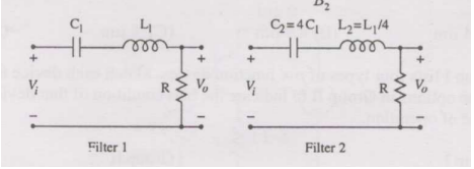
\includegraphics[width=\columnwidth, height=0.8\textheight, keepaspectratio]{fig.png}     


\vspace{0.5em}
\begin{columns}
    \column{0.25\textwidth}\centering (A) 4
    \column{0.25\textwidth}\centering (B) 1
    \column{0.25\textwidth}\centering (C) $\dfrac{1}{2}$
    \column{0.25\textwidth}\centering (D) $\dfrac{1}{4}$
\end{columns}
\end{frame}

%------------------------------------------------------------
\begin{frame}{Theoretical Background}
For a \textbf{series RLC resonant circuit}, the bandwidth is:

\[
B = \frac{R}{L}
\]

\begin{itemize}
\item Bandwidth depends only on:
\begin{itemize}
\item Resistance ($R$)
\item Inductance ($L$)
\end{itemize}

\item It is \textbf{independent of capacitance}
\end{itemize}

\end{frame}

%------------------------------------------------------------
\begin{frame}{Filter 1 Analysis}
For Filter 1:

\[
B_1 = \frac{R}{L_1}
\]

\begin{itemize}
\item $R$ is same for both filters
\item Inductance is $L_1$
\end{itemize}

\end{frame}

%------------------------------------------------------------
\begin{frame}{Filter 2 Analysis}
Given:

\[
L_2 = \frac{L_1}{4}
\]

Bandwidth:

\[
B_2 = \frac{R}{L_2}
\]

Substituting:

\[
B_2 = \frac{R}{L_1/4}
\]

\[
B_2 = \frac{4R}{L_1}
\]

\end{frame}

%------------------------------------------------------------
\begin{frame}{Ratio Calculation}

\[
\frac{B_1}{B_2} = \frac{R/L_1}{4R/L_1}
\]

Canceling common terms:

\[
\frac{B_1}{B_2} = \frac{1}{4}
\]

\end{frame}

%------------------------------------------------------------
\begin{frame}{Important Insight}

\begin{itemize}
\item Capacitance change does NOT affect bandwidth
\item Only inductance scaling matters:
\begin{itemize}
\item $L \downarrow \Rightarrow B \uparrow$
\end{itemize}
\item Since $L_2 = L_1/4$, bandwidth increases 4 times
\end{itemize}

\end{frame}

%------------------------------------------------------------
\begin{frame}{Final Answer}

\[
\boxed{\frac{B_1}{B_2} = \frac{1}{4}}
\]

\end{frame}

%------------------------------------------------------------

\end{document}